\documentclass[tikz,border=2mm]{standalone}

\begin{document}

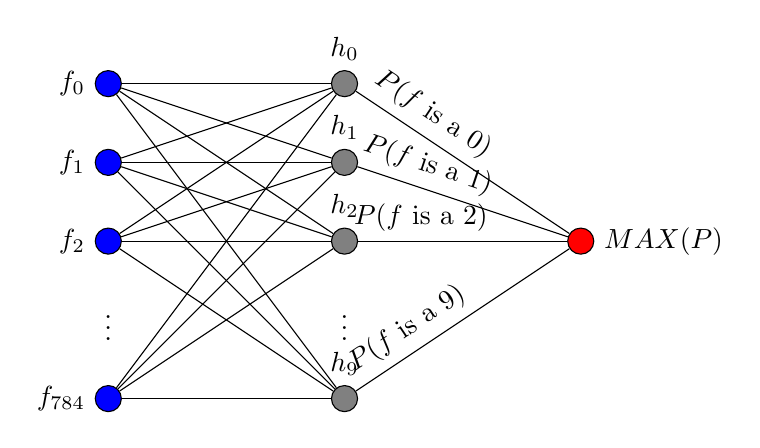
\begin{tikzpicture}
[   cnode/.style={draw=black,fill=#1,minimum width=3mm,circle},
]
    \node[cnode=red,label=0:$MAX(P)$] (s) at (6,-2) {};
    \node at (0,-3) {$\vdots$};
    \node at (3,-3) {$\vdots$};
    \foreach \x in {0,...,3}
    {   \pgfmathparse{\x<3 ? \x : "784"}
        \node[cnode=blue,label=180:$f_{\pgfmathresult}$] (x-\x) at (0,{-\x-div(\x,3)}) {};
    }
    \foreach \x in {0,...,3}
    {   \pgfmathparse{\x<3 ? \x : "9"}
        \node[cnode=gray,label=90:$h_{\pgfmathresult}$] (p-\x) at (3,{-\x-div(\x,3)}) {};
        \draw (p-\x) -- node[above,sloped,pos=0.3] {$P(f \textrm{ is a } {\pgfmathresult})$} (s);
    }
    \foreach \x in {0,...,3}
    {   \foreach \y in {0,...,3}
        {   \draw (x-\x) -- (p-\y);
        }
    }
\end{tikzpicture}

\end{document}
